\chapter{實驗驗證與結果分析}
\label{ch:evaluation}

\section{實驗環境與測試場景設置}
\label{sec:exp_setup}
本節說明驗證本系統所需之軟硬體環境配置，並詳述如何透過虛擬化技術構建符合 3GPP 標準之多用戶實驗拓樸。

\subsection{軟硬體環境配置}
\label{subsec:exp_environment}

本研究之驗證環境分為「實體環境基準測試」與「雲原生編排效能驗證」兩大部分。實體環境基準測試旨在建立未經編排框架介入時的網路效能底線，採用純本地部署方式；雲原生編排驗證則基於 Nephio 平台實施自動化管理與意圖轉譯實作。

表 \ref{tab:hardware_specs} 詳列了本研究使用之硬體設備規格。實體環境驗證（Local Test）運行於具備 Intel Core i7-10700 處理器之主機。而本研究提出之意圖驅動編排系統，其核心平台（Nephio）則部署於另一台具備 Intel Core i5-13500 處理器與 64GB 記憶體之主機，並透過 VirtualBox 虛擬化技術建構實驗環境。該虛擬機（VM）被分配 10 核心 CPU 與 32GB 記憶體，用以承載管理叢集（Management Cluster）與工作負載叢集（Workload Cluster）。

\begin{table}[htbp]
    \centering
    \caption{實驗硬體環境規格}
    \label{tab:hardware_specs}
    \begin{tabular}{|l|l|l|l|}
    \hline
    \textbf{角色} & \textbf{處理器 (CPU)} & \textbf{記憶體 (RAM)} & \textbf{備註} \\ \hline
    實體機測試主機 & Intel Core i7-10700 & 32 GB & 本地環境測試 \\ \hline
    Nephio 宿主機 & Intel Core i5-13500 & 64 GB & 虛擬化底層 \\ \hline
    編排驗證虛擬機 & 10 vCPU & 32 GB & VirtualBox VM \\ \hline
    \end{tabular}
\end{table}

在軟體元件方面，本系統採用 MicroK8s v1.28 作為雲原生基礎設施平台。核心網實作採用 free5GC v4.2.1，無線存取網則基於 srsRAN release\_26\_04 版本。UE則採用官方配套使用的srsRAN 4G 專案中之 srsue v25.10版本，模組編排框架部分採用 Nephio R5，並結合本研究開發之 E2E Orchestrator 進行跨網域編排。表 \ref{tab:software_versions} 摘要了主要軟體元件之版本資訊。

\begin{table}[htbp]
    \centering
    \caption{實驗軟體元件版本資訊}
    \label{tab:software_versions}
    \begin{tabular}{|l|l|l|}
    \hline
    \textbf{軟體元件} & \textbf{軟體名稱} & \textbf{版本}\\ \hline
    容器編排平台 (CISM) & MicroK8s & v1.28\\ \hline
    雲原生編排框架 & Nephio & R5 \\ \hline
    核心網 (5G Core) & free5GC & v4.2.1 \\ \hline
    無線存取網 (RAN) & srsRAN & release\_26\_04 \\ \hline
    用戶設備模擬 (UE Emulator) & srsue submodule in srsRAN 4G & v25.10 \\ \hline
    意圖編排器 & E2E Orchestrator (Golang/Kubebuilder) & \\ \hline
    \end{tabular}
\end{table}

值得注意的是，實體環境驗證採取 Local 部署路徑，網元間直接於 Ubuntu 系統進行對接測試，不涉及 Kubernetes 資源調度和意圖下發流程，以此確保量測數據能真實反映 srsRAN 與 free5GC 在該硬體環境下的原生效能。

\subsection{測試指標與評估定義}
\label{subsec:metrics_definition}

為量化驗證意圖驅動編排系統在資源隔離與自動化流程中之效能，本研究定義了以下兩大類評估指標。第一類針對網路切片之數據面（Data Plane）服務品質保障，第二類則針對管理面（Management Plane）之編排效率。

\subsubsection{數據面服務品質指標 (Data Plane QoS Metrics)}
本研究利用 \texttt{iperf3} 工具產生 UDP 流量，模擬異質業務負載 。透過在用戶設備端之容器命名空間內進行量測，定義以下三項關鍵指標：
\begin{itemize}
    \item \textbf{吞吐量 (Throughput)}：單位時間內成功傳輸之有效位元速率（Bitrate）。
    \item \textbf{封包遺失率 (Packet Loss Rate)}：未成功抵達接收端之數據包占總發送包之比例。此指標為衡量資源隔離有效性之核心，當 eMBB 與 URLLC 產生資源競爭時，系統應優先保障 URLLC 之低遺失率要求 。
    \item \textbf{抖動 (Jitter)}：接收端封包到達時間之變動量。針對延遲敏感型業務（如 URLLC），低抖動是維持通訊穩定之必要條件。
\end{itemize}

\subsubsection{管理面編排效能指標 (Management Plane Metrics)}
為評估本研究基於 Nephio 與 Kubernetes Operator 構建之編排管道效率，本研究定義了「端到端編排時延（End-to-End Orchestration Latency）」。此時延定義為從意圖擁有者下發指令，至實體網元配置生效之總耗時。

依據本系統之工作流，總時延分為以下三個關鍵觀測點：
\begin{equation}
    T_{total} = T_{orchestration} + T_{sync} + T_{operator}
\end{equation}

其中各分項定義如下：
\begin{itemize}
    \item \textbf{編排與轉譯時延 ($T_{orchestration}$)}：定義為從 \texttt{E2EQoSIntent} 套用（$T_0$）至 Nephio Porch 完成套件修改與發佈（$T_1$）之時間。此階段反映了 E2E Orchestrator 之轉譯引擎效率。
    \item \textbf{狀態同步時延 ($T_{sync}$)}：定義為從 Porch 完成發佈（$T_1$）至工作負載叢集之 ConfigSync 完成 Git 資源拉取（$T_2$）之時間。此階段受限於 GitOps 之輪詢週期。
    \item \textbf{領域調和時延 ($T_{operator}$)}：定義為 \texttt{srsran-operator} 監聽到資源變更並生成最終實體 \texttt{ConfigMap}（$T_3$）之耗時。此指標反映了本研究開發之 NSSMF 邏輯執行效率。
\end{itemize}

\subsubsection{意圖達成狀態指標 (Intent Fulfillment Metrics)}
除了量化指標外，本研究亦根據 3GPP TS 28.312 定義之達成狀態（Fulfillment State）作為定性分析依據 。系統會透過 CRD 的 \texttt{status} 欄位回饋 \texttt{FULFILLED} 或 \texttt{NOT\_FULFILLED} 標籤，用以判定網域特定參數（如 5QI 與 PRB Ratio）是否已正確實體化於目標環境中。

\section{端到端切片效能隔離驗證}
\label{sec:slice_performance}
本節透過兩組對照實驗，驗證本系統在不同部署環境下對 eMBB 與 URLLC 切片之資源隔離能力。

\subsection{實驗一：實體環境下之跨網域 QoS 驗證}
\label{subsec:local_qos_verification}

本實驗旨在建立未經雲原生編排框架介入時之網絡效能基準，透過在 Ubuntu 實體主機上直接部署 srsRAN 與 free5GC，驗證 5G 協議棧在無線存取網端實施資源隔離的可行性。本實驗不涉及 Kubernetes 資源調度與意圖轉譯流程，僅作為後續自動化編排之效能對照組。

\subsubsection{實驗設計與環境配置}
本實驗註冊兩組用戶設備（UE），其 IMSI 與切片對應關係如表 \ref{tab:ue_slice_mapping} 所示。在 QoS 參數設定上，eMBB 切片採用 5QI 9（Non-GBR），而 URLLC 切片則配置為 5QI 82（Delay Critical GBR）。

清單 \ref{lst:local_du_config} 展示了本實驗所採用之雙切片排程參數。

\begin{lstlisting}[language=yaml, caption={實體機實驗之 DU 雙切片排程配置參數}, label={lst:local_du_config}]
slicing:
  - # Slice 1: eMBB (5QI=9)
    sst: 1
    sd: 66051
    sched_cfg:
      min_prb_policy_ratio: 0
      max_prb_policy_ratio: 50
      priority: 10

  - # Slice 2: URLLC (5QI=82)
    sst: 1
    sd: 1122867
    sched_cfg:
      min_prb_policy_ratio: 0
      max_prb_policy_ratio: 100
      priority: 200
\end{lstlisting}

\subsubsection{測試程序與流量模型}
本實驗利用 \texttt{iperf3} 工具模擬真實業務負載。為排除外網延遲干擾，測試流量於本機建立之 \texttt{dummy interface} 上運行，並透過網路命名空間（Network Namespace）與 \texttt{bind-dev} 技術強制流量進入 UE 之隧道介面。測試流程定義如下：

\begin{enumerate}
    \item \textbf{階段一 (0--15s)}：啟動 eMBB 流量測試（UE1），設定為 5 Mbps 之 UDP 負載。
    \item \textbf{階段二 (15--45s)}：於第 15 秒加入 URLLC 流量測試（UE2），設定為 1 Mbps 之 UDP 負載，模擬異質切片競爭無線資源之情境。
    \item \textbf{階段三 (45--60s)}：於第 45 秒停止 URLLC 流量，觀察 eMBB 業務之恢復情形。
\end{enumerate}

\subsubsection{實驗結果分析}
實驗結果如圖 \ref{fig:urllc_vs_embb_result} 所示。透過時序圖表可觀察到系統在不同階段之效能特徵：在階段一（0--15s），僅有 eMBB 運行時，流量可吃滿預設頻寬且維持極低之掉包率。進入階段二（15--45s）後，隨 URLLC 流量加入，srsRAN 排程器依據清單 \ref{lst:local_du_config} 之優先級定義，優先保障 URLLC 之傳輸，使其吞吐量與延遲幾乎不受影響；相對地，eMBB 之 PRB 資源受限，導致其 Loss Rate 與 Jitter 值顯著飆高。進入階段三（45s 後），隨 URLLC 流量結束，eMBB 立即恢復至正常效能水平。
值得注意的是，eMBB 之掉包率在競爭初期（15--40s）並未立即上升，主要係因 srsRAN L2 緩衝區（Buffering）機制使封包仍能按序排隊發送，未產生序號斷層；直至第 40 秒左右因緩衝區溢位或封包超時拋棄機制觸發，導致 \texttt{iperf3} 偵測到大量封包序號中斷，掉包率才呈現爆發性增長。此結果證實了透過修改存取網組態落實雙切片隔離之有效性。

\begin{figure}[htbp]
    \centering
    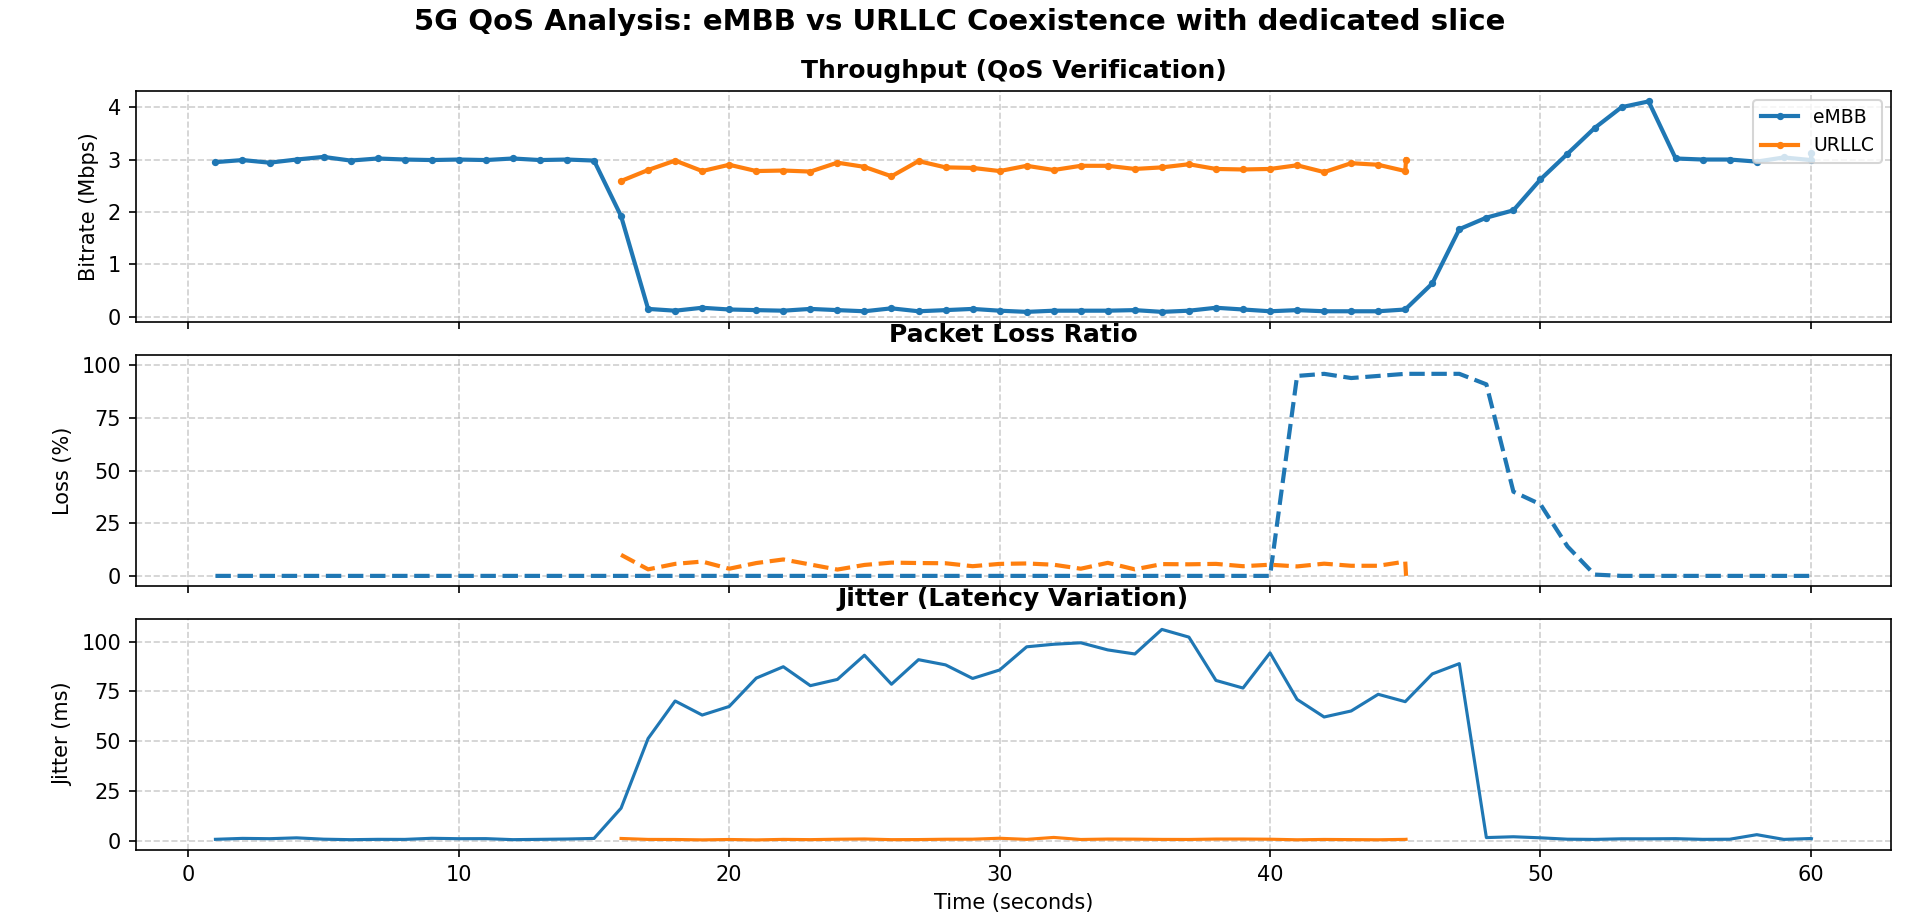
\includegraphics[width=1.0\linewidth]{img/4.2.1-urllc-vs-embb.png}
    \caption{實體環境下 eMBB 與 URLLC 切片之效能競爭與隔離分析圖}
    \label{fig:urllc_vs_embb_result}
\end{figure}

\subsubsection{實驗限制討論}
本實驗雖達成預期隔離效果，但受限於以下因素：首先，\texttt{srsue} 為純軟體模擬，需處理極高之信號採樣率與完整之 L1/L2/L3 協議棧，效能高度依賴主機 CPU 運算能力。誠如 srsRAN 官方文檔所述，該模擬器主要用於可行性驗證而非大規模性能壓力測試。其次，由於 free5GC 之 \texttt{gtp5g} 模組尚未實作不同 5QI 之優先級發送功能，因此目前的隔離效果完全仰賴於 srsRAN 端之排程配置，核心網端尚未具備主動之 QoS 優先發送機制。

\subsection{實驗二：Nephio 雲原生部署之一致性驗證}
\label{subsec:k8s_qos_consistency}

在確立實體環境之效能基準後，本實驗旨在驗證本系統於雲原生環境下，透過 Nephio 自動化編排框架實施切片資源隔離之一致性。本實驗將 5G 網元部署於基於 MicroK8s 之虛擬化環境中，並由 E2E Orchestrator (NSMF) 進行意圖轉譯與參數下發，藉此評估雲原生架構對網路切片效能之影響。

\subsubsection{實驗設計與環境優化策略}
本實驗之網元部署完全遵循第 \ref{sec:ran_nssmf_implementation} 節所述之 Nephio 工作流。實驗註冊兩組用戶設備（UE），其配置與 3GPP 參數對應關係維持與實驗一一致。

考量到工作負載叢集運行於 VirtualBox 虛擬機環境，虛擬化層級之介入易導致頻繁之內核上下文切換（Context Switch），進而引發 CPU 使用率異常飆升與網元效能下降。為此，本研究在 srsRAN 之 \texttt{expert\_execution} 參數中引入了優化配置，如清單 \ref{lst:vm_optimization} 所示。透過調整執行緒之退避週期（Backoff Period），有效緩解了虛擬化環境下之運算壓力，確保模擬器之協議棧能在受限資源下維持穩定運作。

\begin{lstlisting}[language=yaml, caption={針對虛擬化環境之 srsRAN 執行緒優化配置}, label={lst:vm_optimization}]
expert_execution:
  threads:
    main_pool:
      backoff_period: 1000
\end{lstlisting}

\subsubsection{測試程序與流量實施}
測試流程採用與實驗一相同之三階段模型（0--15--45--60s）。為精確模擬容器環境下之業務接入，本研究利用 \texttt{nsenter} 工具穿透容器邊界，進入 UE Pod 專屬之網路命名空間，並將 \texttt{iperf3} 流量綁定於隧道介面 \texttt{uesimtun0}。受測流量之目標端點為部署於 UPF Pod 內之虛擬介面，以排除外部網路之不確定變因。

\subsubsection{實驗結果分析與討論}
實驗結果如圖 \ref{fig:k8s_urllc_vs_embb} 所示。整體效能走勢與實體環境實驗（實驗一）展現高度一致性：
\begin{itemize}
    \item \textbf{資源競爭行為}：在第 15 秒加入 URLLC 流量後，系統能精確落實由 Nephio 編排之 PRB 優先級政策。數據顯示 URLLC 流量能穩定維持在約 1.42 Mbits/sec 的傳輸速率，而 eMBB 則因資源被奪取而導致吞吐量大幅下降至約 215 Kbits/sec，且伴隨明顯之延遲抖動上升。
    \item \textbf{虛擬化損耗評估}：受限於 VM 與 Kubernetes 網路層（Multus/CNI）之封裝開銷，本實驗之最大可用吞吐量設定為 1.5 Mbps，較實體機之 3 Mbps 為低。這證實了在雲原生環境下，雖然資源隔離邏輯（PRB/Priority）能正確實施，但底層虛擬化與 CISM 平台之介入確實會引入額外之處理成本。
    \item \textbf{隔離有效性確認}：儘管絕對流量值受限，但在 45 秒 URLLC 流量結束後，eMBB 之吞吐量隨即恢復至 1.5 Mbps 以上之水準，證明本研究開發之二層編排架構能確保宣告式意圖在動態變化的容器環境中仍能維持最終一致性之資源保障。
\end{itemize}

\begin{figure}[htbp]
    \centering
    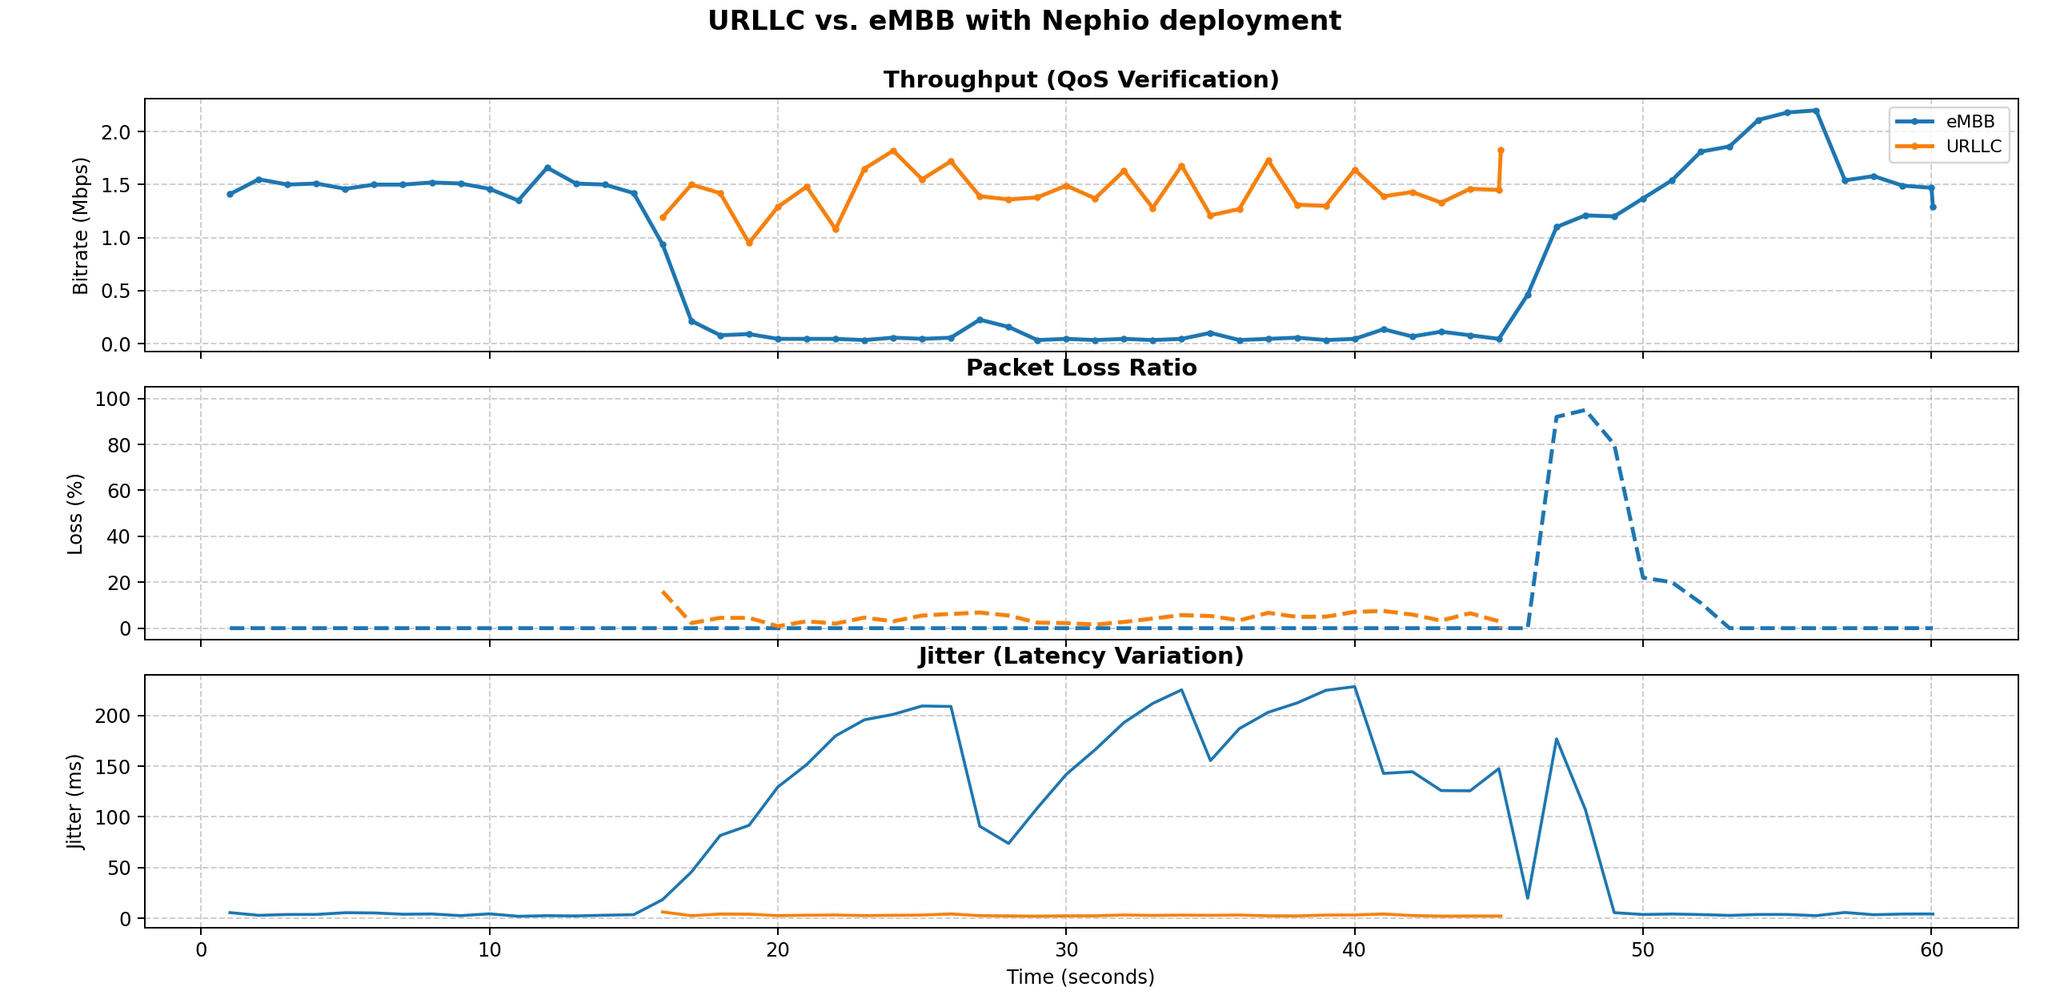
\includegraphics[width=1.0\linewidth]{img/4.2.2-urllc-vs-embb.png}
    \caption{Nephio 雲原生環境下之雙切片效能驗證與隔離分析圖}
    \label{fig:k8s_urllc_vs_embb}
\end{figure}

綜上所述，實驗二驗證了本系統具備跨環境之配置一致性。這代表透過 E2E Orchestrator 對 Nephio Porch 進行自動化套件生命週期管理（Mutation/Approve），能如同手動配置般精確地驅動 NSSMF (Operator) 達成存取網域之 QoS 隔離目標。

\section{意圖驅動編排效率評估}
\label{sec:orchestration_efficiency}
本節旨在量化評估本編排架構在電信雲自動化流程中之時效性能。

\subsection{實驗三：編排工作流時延分析}
\label{subsec:latency_analysis}
透過量測從 Intent apply 至實體網元配置生效（ConfigMap 更新）之端到端時延，評估 NSMF 與 Provisioning MnS Framework 之運作效率。

\subsection{階段耗時分解與討論}
針對意圖轉譯、GitOps 同步以及 Operator 執行等不同階段之時延進行拆解分析，並探討系統之擴展性。

\section{意圖自動化轉譯與自癒功能驗證}
\label{sec:functional_validation}
本節針對編排系統之功能正確性進行定性分析。

\subsection{轉譯引擎準確性分析}
驗證 SLA 期望指標是否能精確映射為 3GPP 定義之 5QI 參數與 RAN 網域之 PRB 比例。

\subsection{狀態回饋與自癒閉環驗證}
展示系統如何透過 CRD Status 追蹤意圖達成狀態，並在配置漂移時透過控制迴圈（Control Loop）達成自動化修復。

\section{本章小結}
總結實驗結果，確認本研究提出之架構能有效簡化切片管理門檻並保障端到端服務品質。
